\section{Methods}
\subsection{Bidirectional transfer functions model for multi-modal registration}\label{sec:syn_em}

Let $I$, $J$ be two images defined over $\Omega_{I}$, $\Omega_{J}$, respectively. We consider $\Omega_{I}, \Omega_{J}$ as the transformed grids $\mathcal{L}_{I}$, $\mathcal{L}_{J}$ associated to $I, J$, under their corresponding grid-to-space transforms $\mathcal{A}_{I}$, $\mathcal{A}_{J}$ (Fig. \ref{fig:syn_overview}). Let $G$ be the set of possible intensity values these images may take (e.g. $G=\left\lbrace 0,1,...,255\right\rbrace$). We aim to find two diffeomorphisms $\phi_{I}:\Omega_{I}\rightarrow \Omega_{R}$ and $\phi_{J}:\Omega_{J}\rightarrow \Omega_{R}$ such that the images get aligned in the reference space $\Omega_{R}$ after warping them under $\phi_{I}^{-1}$ and $\phi_{J}^{-1}$. In other words, for each point $x \in \Omega_{R}$, $I(\phi_{I}^{-1}(x))$ is mapped to $J(\phi_{J}^{-1}(x))$
(Fig. \ref{fig:syn_overview}). Since transformations $\phi_{I}$ and $\phi_{J}$ establish a correspondence between domains $\Omega_{I}$ and $\Omega_{J}$, they also establish a correspondence between intensities of $I$ and $J$, in the sense that the set of pairs $S = \left\lbrace \left( I(\phi_{I}^{-1}(x)), J(\phi_{J}^{-1}(x))\right): x\in\Omega_{R}\right\rbrace$ may be regarded as a set of independent samples from two \textbf{scalar} random variables $\mathbf{I}, \mathbf{J}$, which are related to each other by a joint probability function $P(\mathbf{I}, \mathbf{J} | I, J, \Phi)$ that depends both, on the observed images and the transformations that align them, and can be estimated from $S$. A common approach to handle multi-modal images is to assume the existence of a \emph{transfer function} $F_{I}$ that maps intensities of image $I$ to intensities of image $J$, or the other way around: assume the existence of $F_{J}$ mapping intensities of image $J$ to intensities of image $I$. The choice between using $F_{I}$ or $F_{J}$ is usually made based on the characteristics of the two modalities under consideration. It is important to notice that this assumption of \emph{functional relationship} between the modalities is very strong, and in general is not satisfied. However, similar studies, most notably \cite{Roche1998} have found that the assumption of a functional dependency is not critical in typical multi-modal brain image registration settings. Here, we will assume the existence of both transfer functions:
\begin{equation}\label{eq:intensity_transfers}
    \begin{array}{ccccc}
        F_{I}\left[\mathbf{I}\right] &=& \mathbf{J}\\
        F_{J}\left[\mathbf{J}\right] &=& \mathbf{I}
    \end{array}.
\end{equation}
Under these assumptions, once the correct transformations $\Phi$ are known, images $I, J$ can be obtained from each other by applying the transfer functions:
\begin{equation}\label{eq:SyNEM_gom_ref}
    \begin{array}{ccccc}
        F_{J}\left[J(\phi_{J}^{-1}(x))\right] &=& I(\phi_{I}^{-1}(x)) &+& \eta_{J}(x)\\
        F_{I}\left[I(\phi_{I}^{-1}(x))\right] &=& J(\phi_{J}^{-1}(x)) &+& \eta_{I}(x)
    \end{array}, x\in\Omega_{R},
\end{equation}
where $\eta_{I}, \eta_{J}$ are random fields that account for acquisition noise.

\begin{figure}[H]
\centering
\fbox{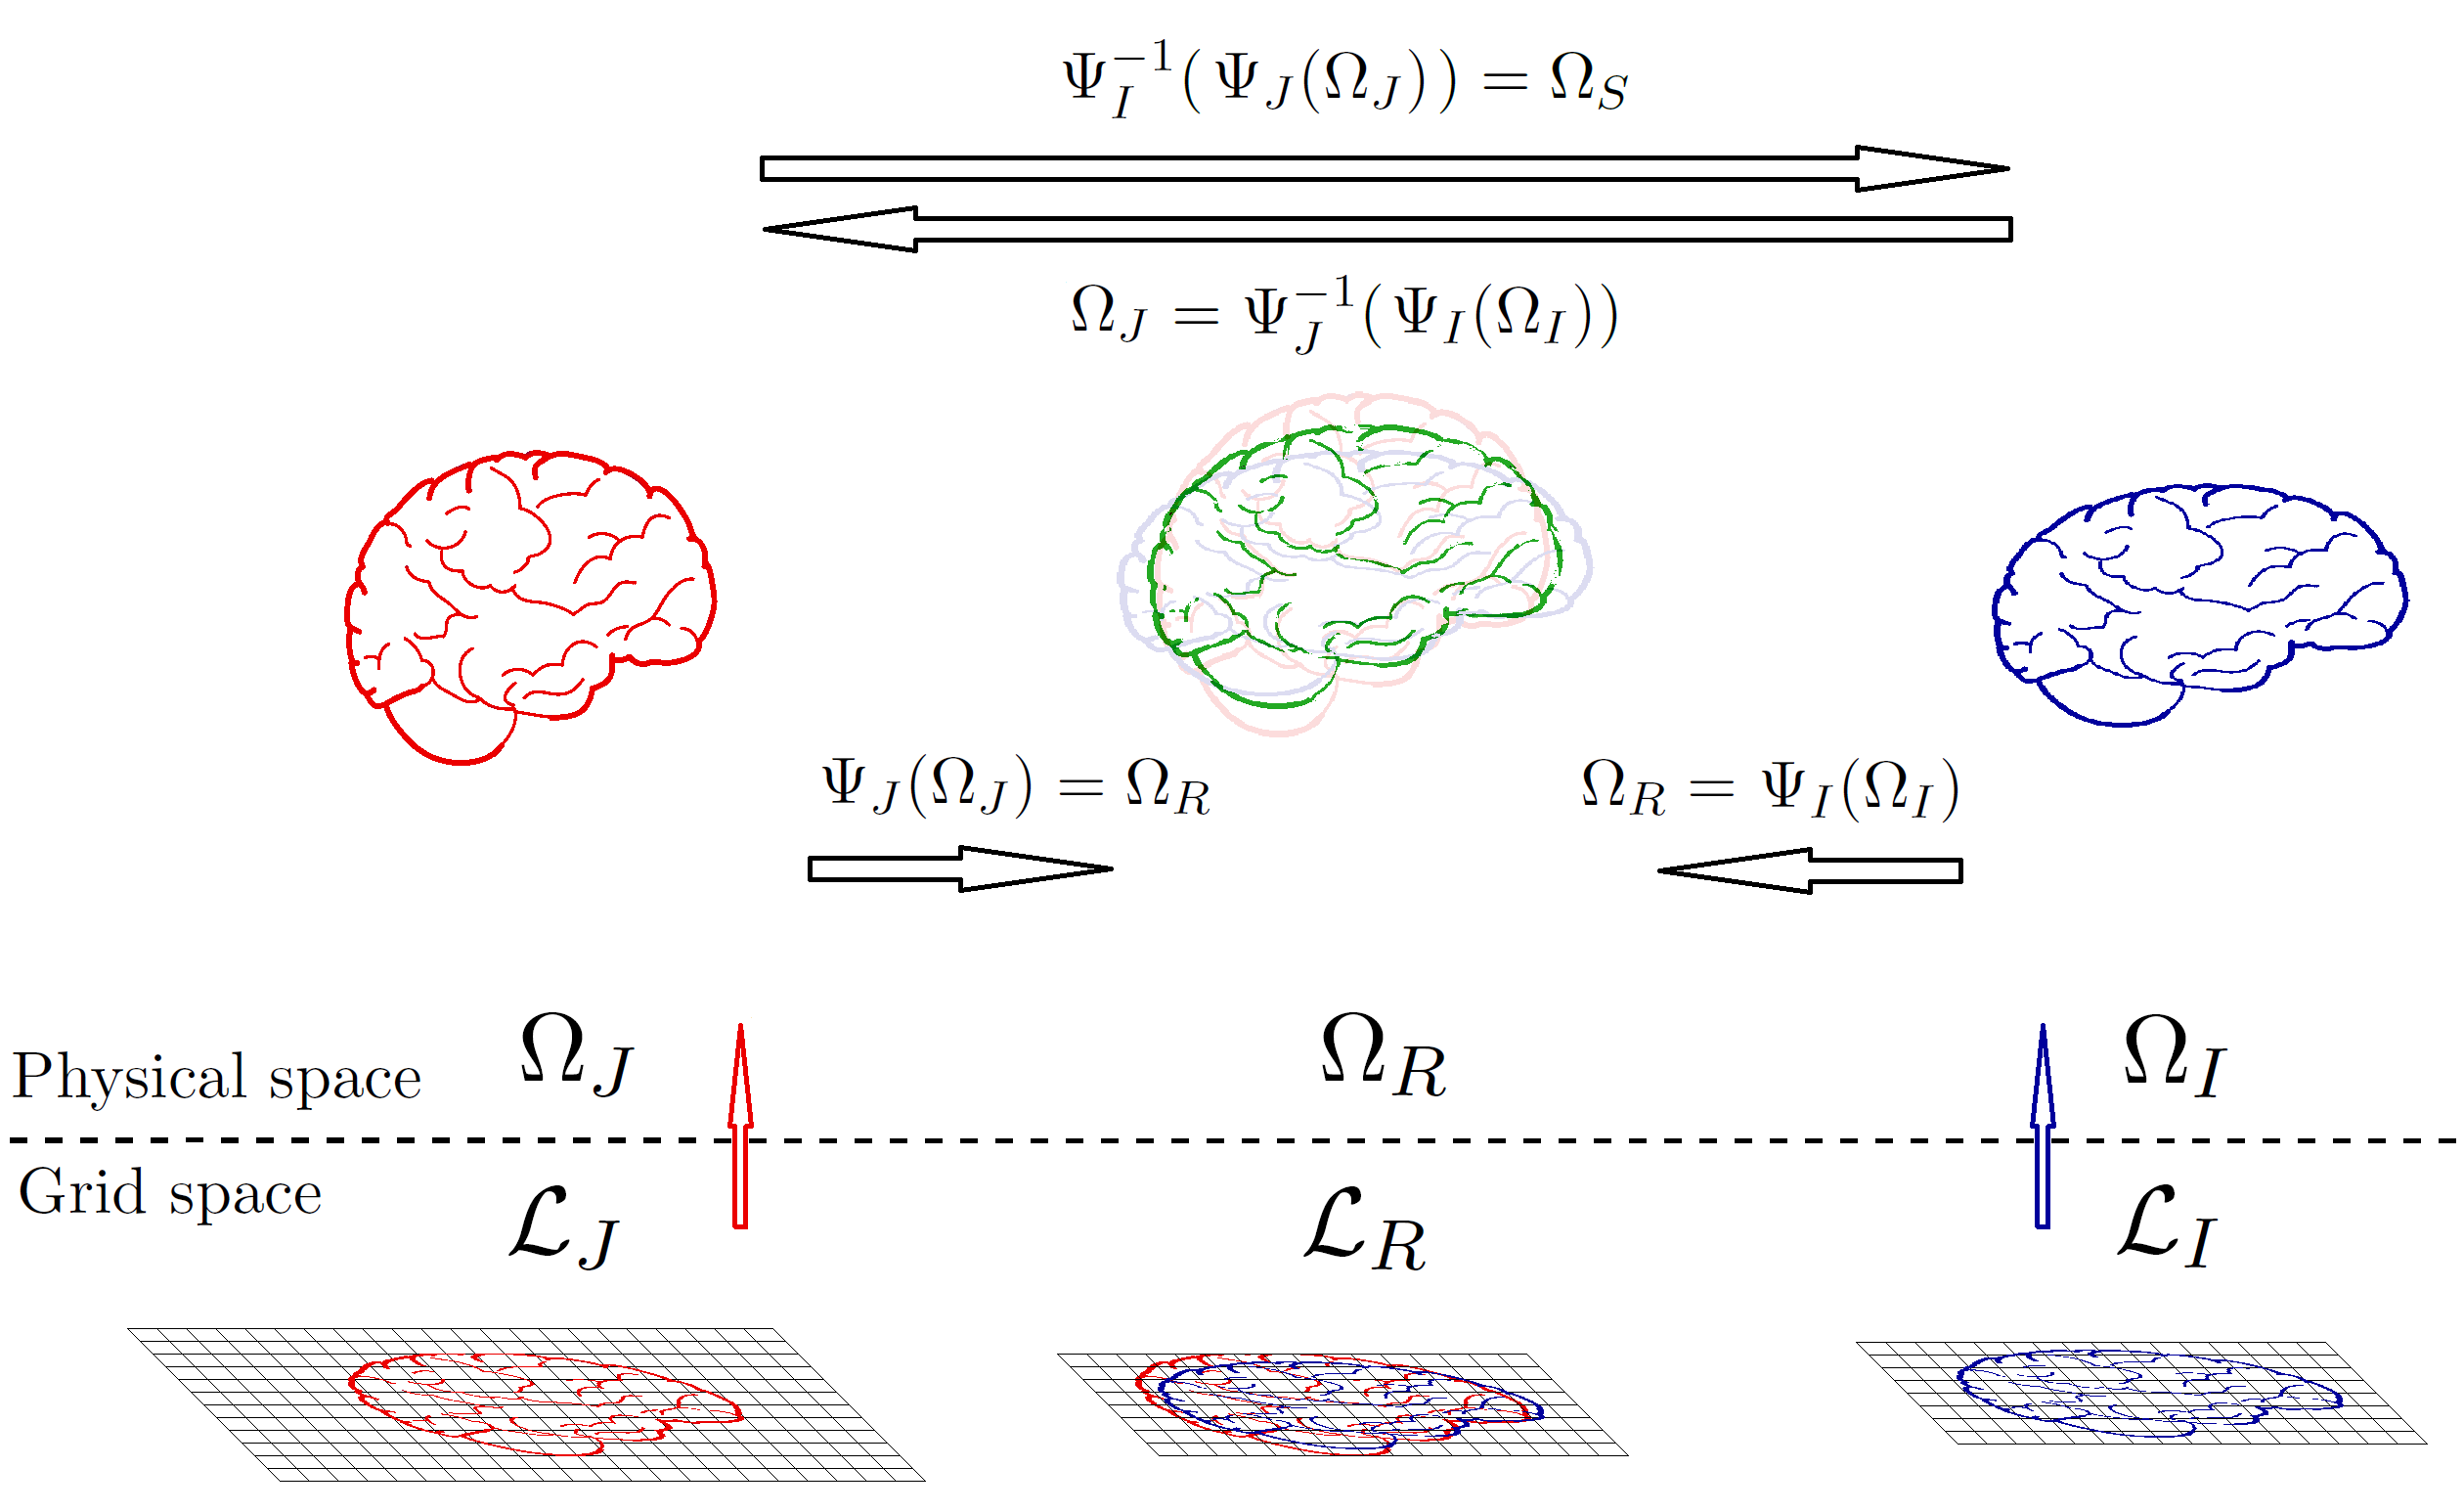
\includegraphics[width=1.0\linewidth]{./images/syn_overview.png}}
\caption{The Greedy SyN algorithm registers two input images by computing two diffeomorphisms that map the input images towards a common reference domain. The final
diffeomorphism is computed by composing the two partial diffeomorphisms.}
\label{fig:syn_overview}
\end{figure}

By defining the warped images \hbox{$\tilde{I}(x) = I(\phi_{I}^{-1}(x))$} and \hbox{$\tilde{J}(x) = J(\phi_{J}^{-1}(x))$} and the hidden random variables \citep{Dempster1977, Li2001}
\begin{equation}\label{eq:hidden_fields}
    \begin{array}{ccc}
        Y(x) &:=& F_{J}\left[\tilde{J}(x)\right]\\[+2mm]
        Z(x) &:=& F_{I}\left[\tilde{I}(x)\right]
    \end{array},x\in\Omega_{R},
\end{equation}
our observation model can be written as
\begin{equation}\label{eq:SyNEM_gom_update}
    \begin{array}{ccccc}
    	Y(x) &=& \tilde{I}(x) &+& \eta_{J}(x)\\
        Z(x) &=& \tilde{J}(x) &+& \eta_{I}(x)
    \end{array}, x\in\Omega_{R}.
\end{equation}
These are precisely two instances of Arce's formulation \citep[see][eq. 1]{Arce-santana2014} in the reference space. The distributions of $Y(x)$ and $Z(x)$ can be written in terms of $\mathbf{I}$ and $\mathbf{J}$ as:
\begin{equation}\label{eq:y_z_i_j_relationship}
    \begin{array}{ccccc}
    	P(Y(x) = i | I, J, \Phi) &=& P(\mathbf{I}=i | \mathbf{J} = J(\phi_{J}^{-1}(x)))\\
        P(Z(x) = j | I, J, \Phi) &=& P(\mathbf{J}=j | \mathbf{I} = I(\phi_{I}^{-1}(x)))\\
    \end{array}, x\in\Omega_{R}.
\end{equation}
Here, we have used the notation $P(\mathbf{I}=i | \mathbf{J} = j)$ instead of \hbox{$P(\mathbf{I}=i | \mathbf{J} = j, I, J, \Phi)$} for simplicity, but it is important to remember that the definition of $P$ depends on $I, J$ and $\Phi$. The conditional expectation and variance of $Y(x)$ given $I, J, \Phi$ can be computed from $P$ as
\begin{equation}\label{eq:expectation_transfer}
    \overline{Y}(x) := \mathbbm{E}\left[\left.Y(x) \right| I, J, \Phi\right] = \mathbbm{E}\left[\left.\mathbf{I} \right| \mathbf{J} = \tilde{J}(x)\right] =
    \int_{\mathbbm{R}} i P(\mathbf{I}=i | \mathbf{J}=\tilde{J}(x)) di
\end{equation}
and
\begin{equation}\label{eq:expectation_variance}
    \sigma_{Y}^{2}(x) := Var\left[\left.Y(x) \right| I, J, \Phi\right] = \int_{\mathbbm{R}} \left(i - \overline{Y}(x)\right)^{2} P(\mathbf{I}=i | \mathbf{J}=\tilde{J}(x)) di.
\end{equation}
Corresponding expressions for $\overline{Z}(x)$ and $\sigma_{Z}^{2}(x)$ are obtained the same way. By performing similar computations as \cite{Arce-santana2014}, we can obtain a symmetric version of the ``EM metric'' to be minimized (named this way since the EM algorithm was used to obtained it), which is the sum of two independent cost functions (see \ref{ap:E_step} for details):
\begin{equation}\label{eq:SyNEM_energy}
    Q(\Phi; \Phi^{(0)}) = Q_{I}(\phi_{I}; \Phi^{(0)}) + Q_{J}(\phi_{J}; \Phi^{(0)})
\end{equation}
given by:
\begin{equation}\label{eq:SyNEM_energy_split}
    \begin{array}{lll}
        Q_{I}(\phi_{I}; \Phi^{(0)}) &=& \sum_{x \in \Omega_{R}} \frac{\left(\overline{Y}(x) - I(\phi_{I}^{-1}(x))\right)^{2}}{2\sigma^{2}_{Y}(x)} + \lambda R(\phi_{I}) \\
        Q_{J}(\phi_{J}; \Phi^{(0)}) &=& \sum_{x \in \Omega_{R}} \frac{\left(\overline{Z}(x) - J(\phi_{J}^{-1}(x))\right)^{2}}{2\sigma^{2}_{Z}(x)} + \lambda R(\phi_{J}) \\
    \end{array}
\end{equation}
where $\Phi^{(0)} = (\phi_{I}^{(0)}, \phi_{J}^{(0)})$ are initial approximations to $\Phi$, and the means and variances of $Y(x)$ and $Z(x)$ are computed using the approximated joint distribution $P(\mathbf{I}, \mathbf{J} | I, J, \Phi^{(0)})$.\\

Notice that $\overline{Y}(x)$ and $\overline{Z}(x)$ are exactly the same optimal transfer functions used in the correlation ratio metric \citep{Roche1998, Roche2000}. Indeed, each of these metrics, derived by \cite{Arce-santana2014}, may be regarded as a generalization of the correlation ratio, which using our notation, is given by \citep[see][eq. 3]{Roche1998}:

\begin{equation}
    CR(I, J, \Phi) = 1 - \frac{Var\left[ \mathbf{I} - \mathbbm{E}\left[ \mathbf{I} | \mathbf{J}\right] \right]}{Var\left[ \mathbf{I} \right]}
\end{equation}
which, in practice, is computed as \citep[see][eq. 4]{Roche1998}:
\begin{equation}
    CR(I, J, \Phi) = 1 - \frac{\frac{1}{|\Omega_{R}|}\sum_{x \in \Omega_{R}} \left(\overline{Y}(x) - I(\phi_{I}^{-1}(x))\right)^{2}}{Var\left[ \mathbf{I} \right]}.
\end{equation}
Therefore, in the special case that all variances $\sigma^{2}_{Y}(x), x\in\Omega_{R}$ are equal, minimizing the EM metric is equivalent to maximizing the correlation ratio metric. The correlation ratio metric arises from an observation model similar to the one presented in \cite{Arce-santana2014}, and extended in this work (eq. \eqref{eq:SyNEM_gom_ref}), but assuming the variance of the noise is constant (see for example eq. 10 in \citep{Roche2000}). However, the EM metric does not make this homoscedasticity assumption, which results in a metric that weighs each squared residual $\left(\overline{Y}(x) - I(\phi_{I}^{-1}(x))\right)^{2}$ using a different factor $\frac{1}{\sigma^{2}_{Y}(x)}$ that measures the uncertainty in the approximation of $\tilde{I}(x)$ by $\overline{Y}(x)$.\\

Functionals $Q_{I}, Q_{J}$ can be efficiently minimized following Vercauteren's analysis of the \textit{diffeomorphic demons} algorithm \citep{Vercauteren2009} as follows.
Let's choose the regularization function $R(\cdot) = ||\nabla \cdot||^{2}$. Starting from the initial transform $\phi^{(0)}_{J}$, we wish to find a small update displacement field $\mathbf{u}$, which minimizes:
\begin{equation}\label{eq:vercauteren_cost}
    \sum_{x \in \Omega_{R}} \frac{\left(\overline{Z}(x) - \tilde{J}(x + \mathbf{u}(x))\right)^{2}}{\sigma^{2}_{Z}(x)} + \lambda ||\nabla \mathbf{u}||^{2}.
\end{equation}

By introducing an auxiliary deformation field $\mathbf{v}$ and a modified energy function
\begin{equation}\label{eq:vercauteren_extended_cost}
    \sum_{x \in \Omega_{R}} \frac{(\overline{Z}(x) - \tilde{J}(x + \mathbf{u}(x)))^{2}}{\sigma^{2}_{Z}(x)} dV + \frac{1}{\tau}||\mathbf{u}-\mathbf{v}||^{2}+\lambda ||\nabla \mathbf{v}||^{2},
\end{equation}
the optimization can be accomplished by alternating two steps. In the first step, we optimize with respect to $\mathbf{u}$ starting with $\mathbf{v} = 0$
\begin{equation}\label{eq:vercauteren_step1}
    \widehat{\mathbf{u}} = \arg\min_{\mathbf{u}}\sum_{x \in \Omega_{R}} \frac{(\overline{Z}(x) - \tilde{J}(x+\mathbf{u}(x)))^{2}}{\sigma^{2}_{Z}(x)} dV + \frac{1}{\tau} ||\mathbf{u}||^{2}.
\end{equation}
We can perform a point-wise minimization by using the first order approximation around the identity
$\tilde{J}(x+\mathbf{u}(x)) \approx \tilde{J}(x) + \nabla \tilde{J}(x)^{T}\mathbf{u}(x)$ and then equating to zero the derivative with respect to $\mathbf{u}(x)$ to obtain:
\begin{equation}\label{eq:euler_lagrange_step1}
    \widehat{\mathbf{u}}(x) = \frac{\overline{Z}(x) - \tilde{J}(x)}{||\nabla \tilde{J}(x)||^{2} + \frac{\sigma_{Z}^{2}(x)}{\tau}}\nabla \tilde{J}(x).
\end{equation}
This expression corresponds to equation (4) in \cite{Vercauteren2009}, but in their work, the factor $\sigma_{Z}^{2}(x)$
is approximated by $\sigma_{Z}(x) \approx |\overline{Z}(x) - \tilde{J}(x)|$ to obtain the traditional {\it demons} step. However, in our case, as in \cite{Arce-santana2014}, we have an explicit and natural estimation of $\sigma^{2}_{Z}(x)$.\\

The second step minimizes eq. \eqref{eq:vercauteren_extended_cost} with respect to $\mathbf{v}$ and keeping fixed the previously obtained displacement field $\mathbf{u}=\widehat{\mathbf{u}}$. The solution of this second sub-problem can be computed by applying a low-pass (smoothing) filter to $\widehat{\mathbf{u}}$. In practice,
this low pass filter is approximated by a Gaussian kernel \citep{Vercauteren2009, Avants2011}.

%To update diffeomorphisms $\phi_{I}, \phi_{J}$ we need to take into consideration that we used their inverses to map images $I, J$ to the reference space. A direct expansion of
%$\tilde{I} \circ \psi$ yields $\phi_{I}^{-1} \leftarrow \phi_{I}^{-1} \circ \psi$, taking its inverse yields $\phi_{I} \leftarrow \psi^{-1} \circ \phi_{I}$, where
%$\psi^{-1} = Id - \mathbf{u}$ for a small displacement field $\mathbf{u}$. We adopted this strategy rather than directly updating the inverses so that the resulting algorithm
%(Alg. \ref{alg:SyNEM})is equivalent to the Greedy SyN algorithm previously described (Alg. \ref{alg:Greedy_SyN}), which has been extensively tested by the neuroimaging
%community.

\subsection{Expected Cross-Correlation}\label{sec:syn_ecc}
The main drawback of using a point-wise metric like SSD, the EM metric previously described, or Mutual Information, is that they are unable to capture important features from the voxels' neighborhood like gradients and texture. Being point-wise, any permutation of the voxels' positions results in exactly the same measured similarity (provided the same permutation is applied to both, the moving and fixed images). This makes point-wise metrics more susceptible to noise and image artifacts such as the bias field in MRI. By considering small windows $W_{y}$ around each voxel $y\in\Omega_{R}$, the normalized Cross Correlation metric (CC), takes advantage of more complex local information, resulting in a more robust metric:
\begin{equation}
    CC(y;\tilde{I}, \tilde{J}) = \frac{\left[\sum_{z\in W_{y}} \left(\tilde{I}(z) - \mu_{y}\right)\left(\tilde{J}(z) - \nu_{y}\right)\right]^{2}}
    {\left[\sum_{z \in W_{y}}\left(\tilde{I}(z) - \mu_{y}\right)^{2}\right] \left[\sum_{z \in W_{y}}\left(\tilde{J}(z) - \nu_{y}\right)^{2}\right]}
\end{equation}
where
\begin{equation}
    \begin{array}{lll}
        \mu_{y} &=& \frac{1}{|W_{y}|}\sum_{z \in W_{y}}\tilde{I}(z)\\
        \nu_{y} &=& \frac{1}{|W_{y}|}\sum_{z \in W_{y}}\tilde{J}(z)\\
    \end{array}.
\end{equation}

The EM formulation belongs to the class of multi-modal image registration methods that reduce the multi-modal problem to a mono-modal one \citep{Sotiras2013}. One of the advantages of this class of methods is that it is relatively easy to extend other mono-modal metrics to the multi-modal case using the same ideas. In particular, we can extend the CC metric for multi-modal images by defining the {\it Expected Cross Correlation} metric as:
\begin{equation}\label{eq:ecc_metric}
    ECC(y;\tilde{I}, \tilde{J}) = CC(y; \overline{Y}, \tilde{I}) + CC(y; \overline{Z}, \tilde{J})
\end{equation}

The first term measures the similarity between $\overline{Y}$ and $\tilde{I}$ (corresponding to a similarity measure in the modality of $I$), while the second term measures the
similarity between $\overline{Z}$ and $\tilde{J}$ (corresponding to a similarity measure in the modality of $J$). The resulting algorithm (see \ref{ap:Algorithms}, alg. \ref{alg:SyNECC}) is, therefore, a combination of the Greedy-SyN algorithm (\ref{alg:Greedy_SyN}) and the SyN-EM algorithm (see \ref{ap:CC_gradient} for details on
computing the gradients).


\subsection{Experiments}
Validation is one of the most challenging aspects of developing image registration algorithms. In order to rigorously evaluate the performance of non-linear
image registration algorithms, we would require a ground-truth consisting of true correspondences between voxels of realistic pairs of images. Since such a ground-truth data are not currently available, researchers resort to surrogates that indirectly measure the quality of their algorithms. For brain MRI registration, for instance, one of the most accepted surrogate measures, is based on the overlap of localized anatomical areas of registered images: ideally, corresponding anatomical areas of perfectly registered images should perfectly overlap. Even a perfect registration algorithm is unlikely to achieve such an ambitious goal, though, since anatomical areas are usually defined manually by an expert, which is by no means a perfect process and the annotations may vary even between different experts. Despite this limitation, it has been shown that among the alternative surrogate measures usually employed, overlap scores of localized anatomical areas is the one that better distinguish reasonable from inaccurate registrations \citep{Rohlfing2012} and it has been employed in the most rigorous evaluations of registration algorithms \citep{Klein2009, Klein2010, Rohlfing2012}. In our experiments, we employ the publicly available Internet Brain Segmentation Repository (IBSR) database consisting of 18 manually annotated T1 brain MRI volumes. Our algorithms are publicly available from the Dipy non-linear registration module \citep{Garyfallidis2014}.\\ 

The methods under evaluation in this section are: 1) SyN with the Normalized Cross Correlation metric \citep{Avants2008, Avants2011}, denoted ``SyN-CC'', 2) SyN with the Mutual Information metric \citep{Mattes2003, Avants2011}, denoted ``SyN-MI'', available in the ANTs software package, 3) the SyN-EM algorithm (see \ref{ap:Algorithms}, alg. \ref{alg:SyNEM}) proposed in section \ref{sec:syn_em}, and 4) the SyN-ECC algorithm (see \ref{ap:Algorithms}, alg. \ref{alg:SyNECC}) proposed in section \ref{sec:syn_ecc}. 